\documentclass[aps,prxquantum,twocolumn,superscriptaddress,amsmath,amssymb,longbibliography,floatfix]{revtex4-2}

\usepackage{graphicx}
\usepackage[colorlinks=true,linkcolor=blue!60!black,citecolor=blue!60!black,urlcolor=blue!60!black]{hyperref}
\usepackage{booktabs}
\usepackage{xcolor}
\usepackage{listings}
\usepackage{amsthm}

\newtheorem{proposition}{Proposition}

\lstset{
  basicstyle=\ttfamily\scriptsize,
  breaklines=true,
  frame=single,
  columns=fullflexible,
  backgroundcolor=\color{gray!5}
}

\begin{document}

\title{An Evidence-First Reproducibility Capsule for NISQ Benchmarking}

\author{Noah Erlwein}
\thanks{ORCID: \href{https://orcid.org/0009-0008-7142-5475}{0009-0008-7142-5475}}
\email{noah@invariantsystems.io}
\affiliation{Invariant Systems}

\date{May 1, 2026}

\begin{abstract}
We introduce an evidence-first reproducibility capsule for NISQ benchmarking that binds logical workload bytes, SHA256 workload identity, provider job IDs, an author-preserved evaluation plan, negative controls, and replayable public analysis into a single auditable release. We demonstrate that contract on an IBM Quantum corpus comprising 33~CHSH runs, a public-bundle expansion campaign containing 168~S1 offline distributions across 28~complete six-backend workload kinds, and a 40-run confirmatory S2 subset. Within that contract, the IBM-only empirical case study yields pairwise Spearman rank correlations across the 6~IBM backends with mean $\bar{\rho} = 0.84$; deterministic permutation sensitivity retains Bonferroni significance for 14/15~backend pairs, while the analytic Spearman t-approximation gives 15/15~significant pairs and identifies the weakest pair as borderline under permutation. Leave-one-family-out recomputation keeps mean $\bar{\rho}$ in $[0.77,\,0.89]$, and residualized rank correlations remain strongly positive after adjusting for width, logical depth proxy, and family. The corresponding empirical claim is deliberately narrow: within this IBM-only corpus, shallow workloads exhibit a stable workload-ordering regularity rather than hardware-independent difficulty. A simple depolarizing-plus-readout model (Proposition~1) matches observed CHSH~$S$ within 3\% on 3 of 6~backends and fails on the remaining three, making it a useful stress test rather than a complete account of device behavior, while readout-error mitigation diagnoses a substantial readout-error contribution on the anomalous backend (\texttt{ibm\_torino}) without elevating the product-state negative controls. A companion AWS Braket confirmation set shows that the same evidence-capture pattern can be exercised on a second real-hardware provider surface, but it is not part of the IBM correlation statistics and does not turn this paper into a matched multi-vendor study. The contribution is a public evidence contract and replayable IBM corpus, not a quantum-advantage, fault-tolerance, provider-attestation, independently preregistered, post-transpilation-identity, or multi-vendor universality claim.
\end{abstract}

\maketitle

%%% ---------------------------------------------------------------
\section{Introduction}
\label{sec:intro}

How much of NISQ performance variation is intrinsic to the circuit, and how much is an artifact of the particular device? This question has practical consequences for benchmarking, error mitigation, and algorithm selection; yet existing frameworks often report device- or suite-level scores without enough public evidence binding for an outside reader to verify what workload ran, where it ran, how it was scored, and what the preserved evaluation plan actually allowed. We address both problems, but the primary contribution here is the evidence-standard one: a reviewer should be able to inspect the public workload bytes, job provenance, decision gates, negative controls, and preserved plan surface rather than infer them from prose. Within that contract, we report a narrower IBM-only empirical case study. For shallow circuits ($\text{depth} \lesssim 20$) on IBM superconducting processors, pairwise Spearman rank correlations across 6~backends and 28~complete six-backend workload kinds (including fixed-parameter structured VQE/QAOA probes, mirror circuits, GHZ-7, Grover search, QFT, and random circuits) yield $\bar{\rho} = 0.84$. Deterministic permutation sensitivity retains Bonferroni significance for 14/15~backend pairs; the analytic Spearman t-approximation gives 15/15~significant pairs, with the weakest pair borderline under permutation. In other words, the performance \emph{ranking} of workloads is largely preserved across the tested IBM devices: relatively difficult workloads tend to remain relatively difficult, and relatively easy workloads tend to remain relatively easy, even though absolute fidelities differ by an order of magnitude.

This IBM-only empirical result emerges from an evidence-first framework for auditable NISQ benchmarking in which workloads are content-addressed (OpenQASM~+~SHA256 identity), evaluation criteria are preserved in an author-maintained plan shipped with the release, and all artifacts suffice for third-party audit. The release also bundles a short companion AWS Braket confirmation note showing that the same evidence-capture pattern can be exercised across a second real-hardware provider surface, but the statistical evidence presented here is IBM-only. The dispute over Google's quantum supremacy claim~\cite{Arute2019} illustrates the auditability gap: the debate centered on whether the classical baseline was fairly specified and whether the quantum computation was adequately characterized. Content-addressed workload identity and an author-dated evaluation-plan surface~\cite{Nosek2018} target exactly that class of auditability problem.

Beyond the cross-backend correlation result, we contribute complementary analyses: reviewer-facing sensitivity checks showing that the IBM-only ranking signal survives family/workload deletion and simple covariate adjustment; a depolarizing noise-model stress test (Proposition~1) that matches observed CHSH~$S$ within 3\% on 3 of 6~backends and fails on the remaining three; and readout-error mitigation that diagnoses a substantial readout-error contribution on the sole anomalous backend.

\textbf{Contributions.} This paper makes four contributions.
\begin{enumerate}
  \item We define an evidence contract for NISQ benchmarking that binds exact logical workload bytes, SHA256 workload identifiers, provider job IDs, author-preserved decision rules, negative controls, and public replay artifacts.
  \item We release a reviewer-recomputable public corpus spanning CHSH, mirror, GHZ, Grover, QFT, random-circuit, and fixed-parameter structured VQE/QAOA probes on real IBM hardware.
  \item We demonstrate the contract on an IBM-only case study by quantifying cross-backend workload-ranking structure across 28 complete six-backend workload kinds within the IBM corpus, showing that deterministic permutation sensitivity retains 14/15 Bonferroni-significant backend pairs while the analytic Spearman test gives 15/15 and identifies the weakest pair as borderline under permutation.
  \item We pair the headline correlations with reviewer-facing diagnostic and sensitivity checks: negative controls, a gate-plus-readout noise model, readout mitigation, GHZ scaling, bootstrap confidence-interval validation, leave-one-family/workload analyses, family-clustered bootstrap, and residualized rank correlation. This keeps failures, anomalies, and robustness limits visible rather than hidden.
\end{enumerate}

\textbf{Key definitions.} By an \emph{evidence-ready NISQ benchmarking posture} we mean the capability to run a declared workload matrix while producing evidence artifacts sufficient for audit, noise-model comparison, and repeatable evaluation. Workloads are identified by their exact OpenQASM bytes plus a SHA256 digest (\emph{logical content-addressed identity}). Hardware outputs are treated as observations, not deterministic functions (\emph{oracle outputs}). Evaluation metrics and decision rules are preserved in an author-maintained evaluation plan (\emph{author-preserved evaluation plan}); negative results are first-class outputs. Throughout, CI95 denotes a 95\% confidence interval and $N$ denotes the shot count. We do not claim determinism of quantum measurement outcomes, provider-signed attestation, independent preregistration, post-transpilation identity, or universal performance improvements across devices.

%%% ---------------------------------------------------------------
\section{Related Work}
\label{sec:related}

Quantum benchmarking has produced several established metrics, each addressing a different facet of device characterization. Our contribution is orthogonal: we propose an \emph{evidence posture} that wraps any workload/metric pair in auditable, content-addressed provenance.

\textbf{Single-number device metrics.} Quantum Volume~\cite{Cross2019} condenses device capability into a single number. CLOPS~\cite{Wack2021} measures execution throughput. Both are useful for coarse ranking but do not specify how results should be identified, archived, or audited by third parties.

\textbf{Randomized benchmarking.} Randomized benchmarking~\cite{Emerson2005,Knill2008,Magesan2011} estimates average gate error rates. Mirror circuits~\cite{Proctor2021} provide holistic fidelity estimates. We include mirror circuits in our corpus (Sec.~\ref{sec:corpus}) but emphasize the \emph{evidence contract} rather than the estimation method.

\textbf{Cross-platform suites.} SupermarQ~\cite{Tomesh2022} and the QED-C suite~\cite{Lubinski2023} define application-oriented benchmarks. Neither requires a public author-declared evaluation-plan surface, per-run shot distributions for offline recomputation, or content-addressed workload identity with Merkle-verifiable provenance as a release requirement. Our differentiator is the combination of a \emph{declared evaluation-plan surface}, \emph{content-addressed identity}, and \emph{execution-level provenance} as public ancillary artifacts; our evidence contract (Sec.~\ref{sec:evidence}) can wrap either suite as an inner workload. We note that this wrapping has not been empirically demonstrated in the present work; validating the framework with SupermarQ or QED-C workloads is planned as future work.

\textbf{Application-oriented benchmarks.} QASMBench~\cite{Li2022qasmbench} provides a curated suite of QASM programs spanning multiple application domains with cross-platform execution. Our framework differs in three ways: (i)~we preserve an explicit evaluation-plan surface with decision rules, (ii)~we publish per-run shot distributions for offline recomputation, and (iii)~logical workload identity is content-addressed (SHA256) rather than filename-based. Our evidence contract (Sec.~\ref{sec:evidence}) could wrap QASMBench circuits as inner workloads.

\textbf{Reproducibility.} Recent work~\cite{Proctor2022} highlights reproducibility challenges in quantum computing. Our framework addresses these directly: workloads are public, analyses are recomputable from published distributions, and negative results are first-class outputs.

\textbf{Error mitigation.} Zero-noise extrapolation (ZNE)~\cite{Temme2017}, probabilistic error cancellation (PEC)~\cite{Li2017}, and matrix-free measurement mitigation (M3)~\cite{Nation2021} have become standard tools for improving NISQ results. We incorporate M3-style readout mitigation as a diagnostic layer (Sec.~\ref{sec:mitigation}) to separate readout error from gate error.

\textbf{Correlated noise.} Crosstalk and temporal correlations on NISQ devices can invalidate independent-shot assumptions~\cite{Sarovar2020}. We address this by comparing IID analytic confidence intervals against non-parametric bootstrap estimates~\cite{Efron1979} (Sec.~\ref{sec:bootstrap}).

\textbf{Reproducibility outside quantum computing.} Preregistration has been advocated as a cornerstone of scientific reproducibility~\cite{Nosek2018}. Content-addressed software deployment (Nix~\cite{Dolstra2006}) provides a model for deterministic, auditable build artifacts. Our framework applies adjacent principles, namely content-addressed identity, explicit evaluation rules, and preserved execution evidence, to quantum workloads.

\textbf{Variational algorithms.} The variational quantum eigensolver (VQE)~\cite{Peruzzo2014} and quantum approximate optimization algorithm (QAOA)~\cite{Farhi2014} are central to the NISQ application thesis. We include fixed-parameter H$_2$ and MaxCut circuits derived from common VQE/QAOA templates not to make variational-optimization claims, but to test whether the evidence framework can carry application-shaped structured circuits alongside the diagnostic families in the IBM-only corpus.

\begin{table*}[t]
\caption{Benchmarking and reproducibility posture. Existing benchmarks answer useful performance questions; the evidence contract in this work specifies the public artifacts needed to audit a benchmark claim.}
\label{tab:benchmark_comparison}
\begin{ruledtabular}
\begin{tabular}{lp{5.0cm}p{6.8cm}}
Framework & Primary role & Evidence-binding distinction \\
\hline
Quantum Volume~\cite{Cross2019} & Single-number device capability threshold & Does not by itself bind public workload bytes, declared decision rules, provider job IDs, and replayable per-run distributions. \\
CLOPS~\cite{Wack2021} & Throughput benchmark for circuit-layer operations & Measures speed rather than fidelity or claim provenance. \\
Randomized benchmarking~\cite{Emerson2005,Knill2008,Magesan2011} & Average gate-error estimation & Characterizes gates but is not a public evidence capsule for application-level workload claims. \\
Mirror circuits~\cite{Proctor2021} & Holistic circuit-fidelity estimation & Supplies useful diagnostic circuits; the present work includes mirror circuits but adds release-level claim gates, job IDs, and replay packaging. \\
SupermarQ~\cite{Tomesh2022} & Application-oriented benchmark suite & Provides scalable workloads and metrics; the present contract can wrap such workloads with a declared plan surface, content addressing, execution IDs, and replay artifacts. \\
QED-C~\cite{Lubinski2023} & Application-oriented benchmark suite and reporting practice & Defines useful benchmark families and aggregate reporting; the present contract emphasizes per-run public distributions, decision gates, and release-local replay. \\
QASMBench~\cite{Li2022qasmbench} & Curated QASM workload corpus & Provides portable logical circuits; the present contract adds provider job IDs, explicit claim boundaries, and recomputable public distributions. \\
This work & Evidence-first NISQ benchmarking capsule & Binds OpenQASM+SHA256 logical workload identity, provider job IDs, declared claim gates, negative controls, public JSON distributions, and replay scripts. \\
\end{tabular}
\end{ruledtabular}
\end{table*}

The difference between the 26-workload submitted S1 manifest and the 28-workload completed public corpus is fully enumerated in the release capsule's scope-reconciliation note. The two additional completed six-backend workload kinds are the historically declared fixed-parameter variational workloads VQE-H$_2$ and QAOA-MaxCut4. The remaining gap relative to the 30-workload planning target is treated as unexecuted planning scope; no headline result uses unexecuted target slots.

%%% ---------------------------------------------------------------
\section{Methods}
\label{sec:methods}

This section states the scientific method and audit boundary needed to interpret the claims in the main text. Exact replay commands, receipt-tooling details, checksum procedures, and provider-specific timestamp surfaces are treated as release-local supplementary material, summarized for reviewers in Table~\ref{tab:replay_map} and the Data and Code Availability section.

\subsection{Workload Identity and Public Corpus}
\label{sec:corpus}

Each workload is referenced by full OpenQASM~2.0 program text and a SHA256 hash over the exact bytes. This binds \emph{logical} workload identity. The present capsule does not bind post-transpilation circuit bytes, transpiler version, optimization level, pulse schedule, or physical qubit layout; those fields should be added for a later multi-vendor or provider-attested release. Table~\ref{tab:corpus_v10} lists the v1.0 core corpus. The v1.1 public-bundle expansion adds 28~workload kinds: mirror depth sweeps ($d{=}1,2,4,8,16$), GHZ-7, Grover (2- and 3-qubit), QFT (4- and 5-qubit), fixed-seed random circuits (widths~4 and~6, depths~8 and~16, seeds~7,~42,~1337,~314159), a fixed-parameter H$_2$ UCCSD circuit ($R = 1.5$\,\AA), and a fixed-parameter MaxCut circuit (4~qubits, $p{=}1$ on the ring graph~$C_4$). These structured circuits use fixed executable angles, making them content-addressed like all other workloads. They are included as application-shaped probes within the evidence contract; no variational-optimization claim is made. Full OpenQASM text and SHA256 IDs for all 28 v1.1 workloads are included in the ancillary files.

\begin{table}[t]
\caption{v1.0 workload corpus. SHA256 is computed over exact OpenQASM bytes (UTF-8, LF).}
\label{tab:corpus_v10}
\begin{ruledtabular}
\begin{tabular}{llp{3.2cm}}
ID & Qubits & SHA256 (first 16 hex) \\
\hline
A1 Bell-2Q   & 2 & \texttt{2fb14387 5ed170f0} \\
A2 GHZ-3Q    & 3 & \texttt{af920034 6cd403c8} \\
A3 GHZ-5Q    & 5 & \texttt{283bcd93 25f1c87b} \\
A4 Mirror-1Q & 1 & \texttt{61eb4f36 dad53e25} \\
\end{tabular}
\end{ruledtabular}
\end{table}

\noindent\begin{minipage}{\columnwidth}
As a concrete example, workload A1 (Bell-2Q) is the following compact OpenQASM program:
\begin{lstlisting}
OPENQASM 2.0;
include "qelib1.inc";
qreg q[2]; creg c[2];
h q[0];
cx q[0],q[1];
measure q -> c;
\end{lstlisting}
\end{minipage}

%%% ---------------------------------------------------------------
\subsection{Author-Preserved Evaluation Plan}
\label{sec:prereg}

We preserve an author-declared evaluation plan covering (i)~a run matrix, (ii)~repetitions, (iii)~shots, and (iv)~a reporting posture that explicitly allows negative outcomes. The full plan, including all metrics, decision rules, the declared workload matrix, and non-claims, is included as an ancillary file (\texttt{PREREGISTRATION\_PUBLIC.json}) so a reader can inspect what was declared for the campaign rather than only the final narrative. The file was not independently timestamped through OSF or a similar registry before execution; accordingly, journal-facing claims in this paper refer to an \emph{author-preserved evaluation plan} rather than preregistration in the metascience sense unless an independent pre-run timestamp is later supplied. No stronger retroactive preregistration claim is made for the present study.

For the CHSH case study, the declared claim gate is: assert violation only when $S > 2.0$ \emph{and} $S_{\mathrm{CI95,low}} > 2.0$ (Section~\ref{sec:chsh}). The CHSH measurement settings use the standard angles: Alice $\theta_a \in \{0, \pi/2\}$, Bob $\theta_b \in \{\pi/4, -\pi/4\}$.

The release also includes an execution-order note summarizing the timestamp posture. In particular, the author-declared plan surface records `date\_declared = 2026-02-01`, later IBM execution artifacts preserve capture-time UTC stamps and IBM Runtime execution-span metadata, and the bundled AWS Braket companion surface preserves provider-native `createdAt` / `endedAt` fields for all eight confirmation tasks. These later timestamps support execution ordering, not independent preregistration of the plan.

\begin{table*}[t]
\caption{Timestamp posture of the main chronology surfaces. Later execution and release timestamps establish ordering of events but do not convert the author-preserved plan into independent preregistration.}
\label{tab:timestamp_posture}
\footnotesize
\begin{ruledtabular}
\begin{tabular}{p{3.0cm}p{3.0cm}p{4.3cm}p{4.3cm}}
Surface & Preserved timing & Supports in this paper & Does not support \\
\hline
\shortstack[l]{\texttt{anc/}\\\texttt{PREREGISTRATION}\\\texttt{\_PUBLIC.json}} & \shortstack[l]{\texttt{date\_declared}\\2026-02-01} & Author-declared pre-execution plan chronology. & Third-party preregistration or registry-backed timestamping. \\
IBM execution evidence & Capture UTC and IBM Runtime execution spans & Execution occurred after the declared plan date. & Registry-style pre-run timestamping of the plan itself. \\
AWS provider facts & Provider-native \texttt{createdAt} / \texttt{endedAt} for all eight IQM Garnet tasks & Second-provider execution ordering and provider-native timing. & Cross-vendor statistical benchmarking or preregistration. \\
Zenodo DOI release & Frozen public release timestamp & Stable public archive identity for the reconciled capsule. & Scientific-evidence dating or an independent pre-execution registry date. \\
\end{tabular}
\end{ruledtabular}
\end{table*}

Table~\ref{tab:scope_reconciliation} reconciles the declared target scope with the completed public evidence scope. The declared plan intentionally remains a historical artifact; completed result claims in this paper use the reconciled public-bundle scope.

\begin{table*}[t]
\caption{Declared-plan and completed-scope reconciliation. The 30-workload / 180-run S1 target is retained as historical planning scope; current result claims use the completed public evidence scope.}
\label{tab:scope_reconciliation}
\begin{ruledtabular}
\begin{tabular}{lccc p{6.3cm}}
Surface & Runs & Workload kinds & Backends & Role in this paper \\
\hline
Declared v1.1 S1 target & 180 & 30 & 6 & Historical author-declared target preserved in \texttt{PREREGISTRATION\_PUBLIC.json}. \\
Submitted v1.1 S1 manifest & 156 & 26 & 6 & Declared submitted-run manifest with binding verification. \\
Completed v1.1 S1 public offline distributions & 168 & 28 & 6 & Reconciled six-backend public corpus used for cross-backend correlation. \\
Confirmatory v1.1 S2 stage & 40 & 10 & 2 & Higher-shot confirmatory subset for S1 stability checks. \\
\end{tabular}
\end{ruledtabular}
\end{table*}

%%% ---------------------------------------------------------------
\subsection{Reproducibility Boundary}
\label{sec:reproducibility}

\subsubsection{Evidence contract}
\label{sec:evidence}

For each executed run we report: backend identifier, provider job~ID, shots, logical workload SHA256~ID, and analysis outputs with confidence intervals where applicable. The evidence contract consists of six steps: (1)~define workloads by content (publish OpenQASM + SHA256 IDs); (2)~declare evaluation rules (publish metrics and decision rules before running); (3)~execute runs (identify each by provider \texttt{job\_id}, backend, and shots); (4)~bind submission identity (manifests include \texttt{submitted\_schedule\_hash}); (5)~publish recomputable data (per-setting distributions for offline verification); (6)~report strict non-claims (only claim what cited artifacts support). Provider job IDs provide job-id provenance but are not provider-signed attestations; parties without provider access can reproduce the logical workload identity (QASM + SHA256), the analysis math, and, for the CHSH case study, recompute~$S$ directly from the per-setting distributions published in this paper. Table~\ref{tab:replay_map} summarizes the reviewer-facing replay surface; exact commands and packaging-tool details remain in the release capsule rather than the main narrative.

\textbf{Companion second-provider hardware confirmation.} The IBM runs form the only statistical corpus analyzed in Sec.~\ref{sec:results}. To test whether the submission and artifact-binding machinery is hard-coded to a single provider surface, we also preserved a bundled non-IBM confirmation set on AWS Braket real hardware. Using the same published logical workloads \texttt{v11\_qft4}, \texttt{v11\_vqe\_h2}, \texttt{v11\_qaoa\_maxcut4}, and \texttt{v11\_grover3}, we executed IQM Garnet at 256 and 4096 shots; all eight Braket tasks completed, and bundled ancillary surfaces now record the task identifiers, provider-side timestamps, logical hash fields, and shot-volume comparison. This confirmation set shows that the same logical workload identities, provider job IDs, and raw-result export pattern survive on a second real-hardware provider surface. It is not part of the IBM cross-backend correlation statistics, does not provide a matched vendor-normalized statistical corpus, and does not establish cross-vendor workload-ranking universality. Azure Quantum submission artifacts from the same campaign are excluded from the real-hardware claim because the attached workspace exposed simulator-only targets at submission time.

\begin{table*}[t]
\caption{Reviewer-facing reproducibility map. Full commands, file paths, and checksum instructions are release-local supplementary material; the table records only the main replay boundary needed for review.}
\label{tab:replay_map}
\footnotesize
\setlength{\tabcolsep}{4pt}
\begin{ruledtabular}
\begin{tabular}{p{3.8cm}p{3.6cm}p{8.3cm}}
Replay step & Output & Expected check \\
\hline
Schema validation & terminal report & \texttt{validate\_ancillaries.py}: 6 ancillary JSON files validate. \\
CHSH recomputation & terminal report & \texttt{verify\_chsh.py}: recomputed $S$ and CI values match the manifest. \\
Cross-backend correlation & correlation JSON & \texttt{cross\_backend\_analysis.py}: 28 workload kinds; deterministic permutation sensitivity 14/15 backend pairs significant; analytic Spearman test 15/15. \\
Readout mitigation & mitigation JSON & \texttt{readout\_mitigation.py}: Bell-state \texttt{ibm\_torino} runs recover; product-state negative control remains below gate. \\
Noise-model comparison & noise-model JSON & \texttt{noise\_model\_comparison.py}: 3/6 backends within 3\% of observed mean~$S$. \\
Scaling diagnostic & scaling JSON & \texttt{scaling\_analysis.py}: descriptive Mirror-to-GHZ-7 exponential diagnostic. \\
\end{tabular}
\end{ruledtabular}
\end{table*}

\subsubsection{CHSH recomputation method}
\label{sec:chsh_method}

For each CHSH run, the measurement uses four settings labeled $\{a_0b_0, a_0b_1, a_1b_0, a_1b_1\}$ with angles $\theta_a \in \{0, \pi/2\}$, $\theta_b \in \{\pi/4, -\pi/4\}$. For each setting, the outcome is a 2-bit string $xy \in \{00, 01, 10, 11\}$ with measured probabilities $P(xy)$.

The parity-based correlation for a single setting is:
\begin{equation}
  E = \sum_{x,y} (-1)^{x \oplus y} \, P(xy) = P(00) - P(01) - P(10) + P(11)
  \label{eq:corr}
\end{equation}
and the CHSH parameter is:
\begin{equation}
  S = E_{a_0b_0} + E_{a_0b_1} + E_{a_1b_0} - E_{a_1b_1}
  \label{eq:chsh}
\end{equation}
Because bit ordering can be ambiguous across systems, we compute~$E$ under both conventions and report both. For the XOR parity observable, both conventions yield identical~$E$ values.

\subsubsection{Uncertainty}

Standard error of each correlation, treating $N$ shots as independent samples of $z \in \{+1, -1\}$ with mean~$E$:
\begin{equation}
  \mathrm{SE}(E) \approx \sqrt{\frac{1 - E^2}{N}}
\end{equation}
Combined standard error and 95\% confidence interval:
\begin{equation}
  \mathrm{SE}(S) = \sqrt{\sum_i \mathrm{SE}(E_i)^2}\,, \quad
  \mathrm{CI}_{95}(S) = S \pm 1.96 \, \mathrm{SE}(S)
\end{equation}

The IID assumption underlying these intervals is validated via bootstrap resampling in Sec.~\ref{sec:bootstrap}.

\subsubsection{Representative CHSH recomputation}
\label{sec:worked}

A representative recomputation is kept release-local rather than expanded into a full in-text probability table. For run~3 (\texttt{job\_id}: \texttt{d5vm0gjuf71s73ciqn30}, backend: \texttt{ibm\_boston}, $N{=}16\,384$), the published per-setting distributions imply $E_{a_0b_0} = 0.698$, $E_{a_0b_1} = 0.697$, $E_{a_1b_0} = 0.691$, and $E_{a_1b_1} = -0.695$, yielding $S = 2.7808$, $\mathrm{SE}(S) \approx 0.0112$, and $\mathrm{CI}_{95} \approx [2.759,\, 2.803]$. These values match Table~\ref{tab:chsh_runs} and illustrate that the headline CHSH result is directly recomputable from the released distributions alone.

%%% ---------------------------------------------------------------
\section{Results}
\label{sec:results}

\subsection{CHSH case study}
\label{sec:chsh}

We select the CHSH test~\cite{Clauser1969,Aspect1982} not for novelty, because Bell-inequality violation on superconducting hardware is well established, but because its sharp classical bound ($S \leq 2$) and well-understood noise sensitivity make it an ideal stress test for the evidence framework: any claim gate must navigate noise, drift, and near-threshold statistics to produce a defensible verdict. CHSH is treated strictly as an entanglement witness measurement with an explicit claim gate: we only assert ``violation observed'' when $S > 2.0$ \emph{and} $S_{\mathrm{CI95,low}} > 2.0$, and only headline it when it replicates across backends.

\textbf{Not a loophole-free Bell test:} we report a CHSH witness measured on NISQ hardware under a declared analysis gate. \textbf{No-signaling sanity:} marginal-deviation deltas are computed under both bit-order conventions and reported as a diagnostic, not a validity gate.

Table~\ref{tab:chsh_runs} summarizes the CHSH results by backend (per-run detail is in the ancillary JSON) and Fig.~\ref{fig:chsh} visualizes the results. Across 26 Bell-state runs, 23 satisfy the declared claim gate ($S > 2.0$ and $S_{\mathrm{CI95,low}} > 2.0$). All 7 product-state negative controls correctly fail the gate. Violations are replicated on five backends (\texttt{ibm\_boston}, \texttt{ibm\_fez}, \texttt{ibm\_kingston}, \texttt{ibm\_marrakesh}, \texttt{ibm\_pittsburgh}); \texttt{ibm\_torino} remains an honest near-threshold/non-violation backend (Bell-state runs in the range $S{\approx}1.94$--$1.98$), reported without exclusion.

\begin{center}
\begin{minipage}{\columnwidth}
\centering
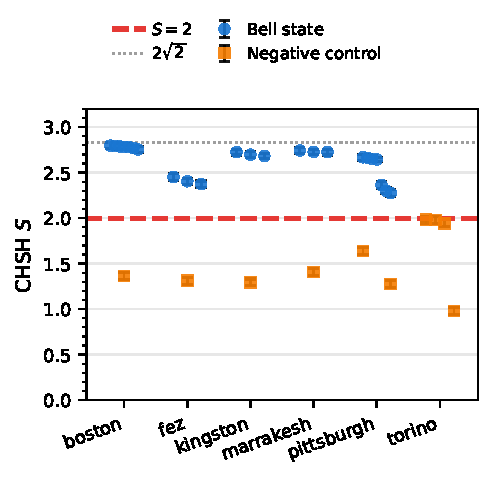
\includegraphics[width=\columnwidth]{fig1_chsh_backends.pdf}

\refstepcounter{figure}\label{fig:chsh}
\small
\textbf{FIG.~\thefigure.} CHSH $S$ values with 95\% confidence intervals, grouped by backend. Blue circles denote Bell-state runs; orange squares denote product-state negative controls. The red dashed line marks the classical bound ($S=2$), and the gray dotted line marks the Tsirelson bound ($S=2\sqrt{2}$). Of 26 Bell-state runs, 23 clear the declared claim gate; 3 near-threshold \texttt{ibm\_torino} runs do not.
\end{minipage}
\end{center}

\begin{table}[tbp]
\caption{CHSH summary by backend (26 Bell-state runs, 7 negative controls; full per-run data in ancillary JSON). $\bar{S}$: mean $S$ over Bell-state runs; $\sigma$: sample standard deviation; $n_{\rm pass}/n$: fraction satisfying the declared claim gate ($S > 2.0$ and $\mathrm{CI95_{low}} > 2.0$). All 7~product-state negative controls correctly fail the gate ($\bar{S}_{\mathrm{ctrl}} \in [0.98,\, 1.64]$). The elevated $\sigma$ for \texttt{ibm\_pittsburgh} reflects runs across two distinct qubit pairs (best-edge and second-best-edge).}
\label{tab:chsh_runs}
\begin{ruledtabular}
\begin{tabular}{lccc}
Backend & $n$ & $\bar{S} \pm \sigma$ & Pass \\
\hline
\textit{Tsirelson bound} & \textit{n/a} & \textit{2.828} & \textit{n/a} \\
\hline
ibm\_boston     & 7 & $2.782 \pm 0.015$ & 7/7 \\
ibm\_fez       & 3 & $2.410 \pm 0.040$ & 3/3 \\
ibm\_kingston  & 3 & $2.703 \pm 0.022$ & 3/3 \\
ibm\_marrakesh & 3 & $2.733 \pm 0.010$ & 3/3 \\
ibm\_pittsburgh& 7 & $2.510 \pm 0.186$ & 7/7 \\
ibm\_torino    & 3 & $1.968 \pm 0.023$ & 0/3 \\
\end{tabular}
\end{ruledtabular}
\end{table}

\subsection{Workload expansion campaign (v1.1 Stage~S1)}
\label{sec:v11}

To address ``toy workload / handcrafted circuit'' critiques, we executed a public-bundle workload expansion consisting of 28~workload kinds across 6~backends at 2\,048~shots per run (Stage~S1). The corpus includes five workload families from the original expansion (mirror, GHZ, Grover, QFT, random circuits) plus two application-shaped fixed-parameter structured circuits declared in the v1.1 planning scope: a VQE-derived H$_2$ circuit~\cite{Peruzzo2014} (2-qubit UCCSD ansatz with the fixed executable angle encoded as \texttt{rz(0.59)} in the published QASM) and a QAOA-derived MaxCut circuit~\cite{Farhi2014} (4-qubit, $p{=}1$ on the ring graph~$C_4$, with fixed executable cost and mixer rotations encoded as \texttt{rz(1.231)} and \texttt{rx(0.7854)} in the published QASM). These are single fixed-parameter workload probes, not variational-optimization experiments or claims about VQE/QAOA algorithmic performance. A later five-backend remediation supplement adds GHZ circuits at $n{=}3$ and $n{=}5$ and a QAOA-v2 rerun for Table~\ref{tab:ghz_grover}; the cross-backend correlation script below uses the 28 workload kinds with complete six-backend public-bundle coverage. Coverage in the bundled S1 offline distributions is 168/168 completed runs, with binding verified and offline distributions available.

\begin{table}[tbp]
\caption{Mirror-1Q return probability $P(0)$ by backend and depth (v1.1~S1, 2\,048~shots). Shot-noise standard error is $\text{SE} \leq 0.007$ for all entries ($\text{SE} = \sqrt{p(1{-}p)/N}$). Depth-independence on most backends is expected for a single-qubit identity-equivalent circuit.}
\label{tab:mirror}
\begin{ruledtabular}
\begin{tabular}{lccccc}
Backend & $d{=}1$ & $d{=}2$ & $d{=}4$ & $d{=}8$ & $d{=}16$ \\
\hline
ibm\_boston     & 1.000 & 1.000 & 1.000 & 1.000 & 1.000 \\
ibm\_fez       & 0.999 & 1.000 & 0.998 & 0.999 & 0.997 \\
ibm\_kingston  & 0.998 & 0.993 & 0.999 & 0.996 & 0.997 \\
ibm\_marrakesh & 0.991 & 0.991 & 0.991 & 0.993 & 0.990 \\
ibm\_pittsburgh& 0.997 & 0.998 & 0.999 & 0.996 & 0.997 \\
ibm\_torino    & 0.909 & 0.909 & 0.907 & 0.914 & 0.920 \\
\end{tabular}
\end{ruledtabular}
\end{table}

Mirror-1Q serves as a \emph{readout-fidelity baseline} rather than a computational benchmark: at any depth, the compiled circuit is identity-equivalent, so $P(0)$ isolates readout error from gate error. This separation is essential for the noise-model analysis in Sec.~\ref{sec:noisemodel}. $P(0)$ remains above~0.99 on 5~of~6 backends across all depths (Table~\ref{tab:mirror} and Fig.~\ref{fig:mirror}); \texttt{ibm\_torino} shows a consistent offset (${\approx}0.91$), consistent with elevated single-qubit readout error on the measured qubit~\cite{Merkel2013}. We report it as-is per the declared posture of including anomalous results without post-hoc exclusion.

\begin{center}
\begin{minipage}{\columnwidth}
\centering
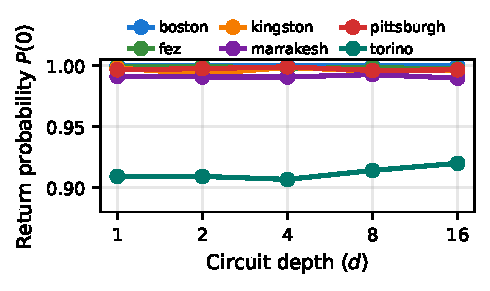
\includegraphics[width=\columnwidth]{fig2_mirror_depth_sweep.pdf}

\refstepcounter{figure}\label{fig:mirror}
\small
\textbf{FIG.~\thefigure.} Mirror-1Q return probability $P(0)$ vs.\ circuit depth by backend. Five of six backends maintain $P(0) > 0.99$ across all depths; \texttt{ibm\_torino} shows a persistent offset.
\end{minipage}
\end{center}

\begin{table*}[t]
\caption{GHZ parity success $P(0^n){+}P(1^n)$ and Grover target-hit $P(1^n)$ by backend (v1.1~S1, 2\,048~shots). Shot-noise SE ranges from $0.005$ (Grover-2) to $0.011$ (GHZ-7). Ideal values from noiseless statevector simulation are shown for comparison.}
\label{tab:ghz_grover}
\begin{ruledtabular}
\begin{tabular}{lccccc}
Backend & GHZ-3 & GHZ-5 & GHZ-7 & Grover-2 & Grover-3 \\
\hline
\textit{Ideal}  & \textit{1.000} & \textit{1.000} & \textit{1.000} & \textit{1.000} & \textit{0.781} \\
\hline
ibm\_boston     & 0.974 & 0.933 & 0.893 & 0.984 & 0.662 \\
ibm\_fez       & 0.934 & 0.841 & 0.504 & 0.795 & 0.662 \\
ibm\_kingston  & n/a   & n/a   & 0.897 & 0.969 & 0.684 \\
ibm\_marrakesh & 0.971 & 0.859 & 0.912 & 0.960 & 0.691 \\
ibm\_pittsburgh& 0.956 & 0.918 & 0.877 & 0.916 & 0.729 \\
ibm\_torino    & 0.793 & 0.699 & 0.708 & 0.794 & 0.643 \\
\end{tabular}
\end{ruledtabular}
\end{table*}

GHZ parity success is lower for larger entangled states on average: mean values are $0.93$ (GHZ-3), $0.85$ (GHZ-5), and $0.80$ (GHZ-7), consistent with per-qubit depolarizing noise (Table~\ref{tab:ghz_grover}). Cross-backend variance grows with $n$: \texttt{ibm\_torino} drops from~0.79 (GHZ-3) to~0.70 (GHZ-5) to~0.71 (GHZ-7), while \texttt{ibm\_boston} maintains $\geq 0.89$ through GHZ-7. Grover target-hit degrades from 2- to 3-qubit as expected. Figure~\ref{fig:heatmap} presents the cross-backend view, showing that performance is workload- and backend-dependent, which is precisely why job-level provenance matters.

\textbf{Cross-backend correlation.} To move beyond data tabulation, we compute pairwise Spearman rank correlations across all 6~backends using the primary metric for each of the 28~public-bundle workload kinds with complete six-backend coverage. Ties are handled by average ranks. The primary sensitivity result is a deterministic 20{,}000-shuffle two-sided permutation test on average ranks with Bonferroni correction across the $\binom{6}{2}=15$ backend pairs: 14/15 backend pairs remain significant, and the weakest pair (\texttt{ibm\_boston}--\texttt{ibm\_torino}, $\rho = 0.54$) is borderline with permutation $p_{\text{Bonf}} = 0.06150$. The analytic Spearman t-approximation ($t = \rho\sqrt{(n-2)/(1-\rho^2)}$, $\text{df}=n-2$) gives 15/15 significant pairs after Bonferroni correction, with the same weakest pair at analytic $p_{\text{Bonf}} = 0.04782$. The mean off-diagonal correlation is $\bar{\rho} = 0.84$ (range: $0.54$--$0.97$), indicating that workload difficulty is \emph{strongly correlated} across most backend pairs (Fig.~\ref{fig:crosscorr}). We note that Spearman rank correlation is invariant to the absolute scale and units of each metric: it tests whether the \emph{ranking} of workload difficulty is preserved across backends, so the heterogeneity of metric types (probabilities, entropies, KL scores, sector fidelities, approximation ratios) does not by itself bias the result. Among the five Eagle~r3 backends, $\bar{\rho} = 0.93$ ($p < 10^{-5}$ for all analytic pair tests), supporting a stable ranking signal within this IBM hardware family. We do not estimate a homogeneity-only null model for these $\rho$ values in this paper, so the result should be read as an empirical regularity within the IBM corpus rather than as proof that workload difficulty is hardware-independent. The highest cross-backend variance occurs for GHZ-7 (coefficient of variation $\text{CV} = 0.20$), confirming that multi-qubit entanglement fidelity is the most device-sensitive metric in our corpus.

\begin{table*}[t]
\caption{Primary workload-family scores used in the cross-backend rank analysis. Each score is a fixed higher-is-better proxy for its own logical workload family; the headline Spearman result tests rank preservation across backends, not interchangeability of the raw metric semantics.}
\label{tab:metric_justification}
\footnotesize
\begin{ruledtabular}
\begin{tabular}{p{2.0cm}p{3.0cm}p{2.8cm}p{3.3cm}p{4.1cm}}
Family & Primary score & Higher means & Main caution & Why acceptable in this corpus \\
\hline
Mirror & $P(0^n)$ & stronger identity return / readout fidelity & dominated by readout bias rather than algorithmic success & used explicitly as a diagnostic baseline rather than an application-level claim \\
GHZ & $P(0^n){+}P(1^n)$ & stronger computational-basis parity success & ignores phase-sensitive structure beyond parity & adequate entanglement-witness proxy for the fixed GHZ workloads in this corpus \\
Grover & $P(1^n)$ & higher marked-state hit probability & oracle- and width-specific score semantics & fixed logical workloads make across-backend ranking comparisons direct \\
QFT & entropy ratio $H/H_{\mathrm{ideal}}$ & output spread closer to the ideal transform & some noise can flatten outputs toward ideal-looking entropy & retained as one diagnostic family rather than as a standalone headline metric \\
Random & normalized KL quality $1 - D_{\mathrm{KL}}/n$ & output spread closer to the expected distribution & some noise can also look more uniform & one family among several; family-drop sensitivity is reported below rather than assumed away \\
VQE & sector fidelity $P(|01\rangle){+}P(|10\rangle)$ & stronger occupation of the expected sector & not an energy estimate or optimization claim & fixed-parameter probe only; used to test whether the ranking signal extends beyond diagnostics \\
QAOA & approximation ratio $\langle C \rangle / C_{\max}$ & stronger fixed-instance cut quality & fixed parameters and shallow depth limit generality & fixed-parameter probe only; not used as an optimization claim \\
\end{tabular}
\end{ruledtabular}
\end{table*}

\subsection{Sensitivity of cross-backend rank structure}
\label{sec:sensitivity}

The headline cross-backend result should be read together with Table~\ref{tab:metric_justification}. Each workload family contributes a fixed higher-is-better score, but the scientific meaning of those scores is family-specific. Spearman correlation is therefore used only to test whether workload \emph{ranking} is preserved across backends, not to assert that the raw metrics themselves are interchangeable or that any one family is sufficient on its own. In this release, that ranking claim is hardened in four additional ways beyond the main permutation sensitivity check.

First, leave-one-family-out recomputation keeps the mean off-diagonal correlation in the range $\bar{\rho} \in [0.77,\,0.89]$. The lowest value occurs when the 16-workload random-circuit family is removed ($\bar{\rho}=0.77$), while removing the five mirror diagnostics increases the mean to $\bar{\rho}=0.89$; no single family deletion collapses the signal. Second, leave-one-workload-out influence checks move $\bar{\rho}$ by at most $\pm 0.021$: omitting \texttt{v11\_grover2} raises the mean to $0.862$, whereas omitting \texttt{v11\_qaoa\_maxcut4} lowers it to $0.822$. These are noticeable leverage effects but not reversals.

Third, a family-clustered bootstrap over the seven workload families yields a conservative 95\% interval $[0.44,\,0.96]$ for mean $\bar{\rho}$ and $[0.14,\,0.98]$ for the weakest observed pair (\texttt{ibm\_boston}--\texttt{ibm\_torino}). The interval is intentionally wide because the family count is small and the random-circuit family contains most workload kinds; this check therefore confirms that the central estimate remains high while making clear that family-level uncertainty is not yet tightly constrained. Fourth, residualized rank correlations that partial out workload width, a QASM-derived logical-depth proxy, and family dummies remain strongly positive across all backend pairs, with mean residualized correlation $\bar{\rho}_{\mathrm{res}} = 0.92$ and pairwise range $[0.85,\,0.97]$. The ranking signal is therefore not explained away by simple width/depth/family covariates alone.

Taken together, these analyses materially strengthen the empirical IBM-only claim: the observed rank structure is not reducible to one family, one workload, or trivial workload covariates. They do \emph{not} eliminate the broader architectural-homogeneity concern discussed below, nor do they substitute for a true multi-vendor corpus.

\begin{figure*}[tb]
\centering
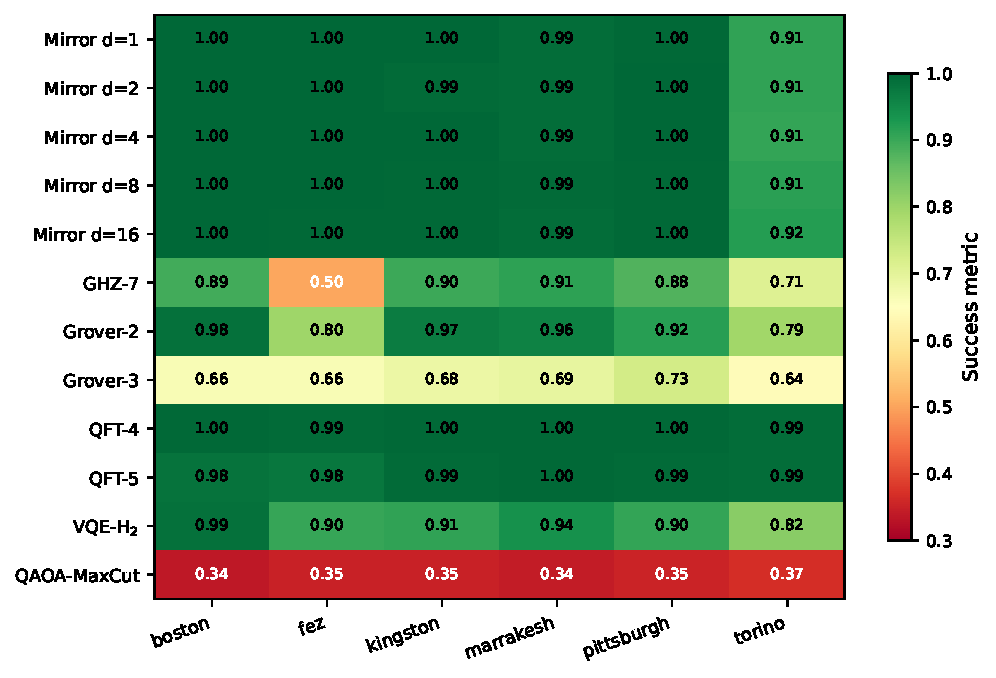
\includegraphics[width=0.92\textwidth]{fig3_v11_heatmap.pdf}
\caption{Cross-backend workload performance heatmap (v1.1~S1, 2\,048 shots). Cell values are the primary success metric for each workload/backend pair. The variation across rows and columns demonstrates that no single backend or workload dominates.}
\label{fig:heatmap}
\end{figure*}

\begin{figure*}[tb]
\centering
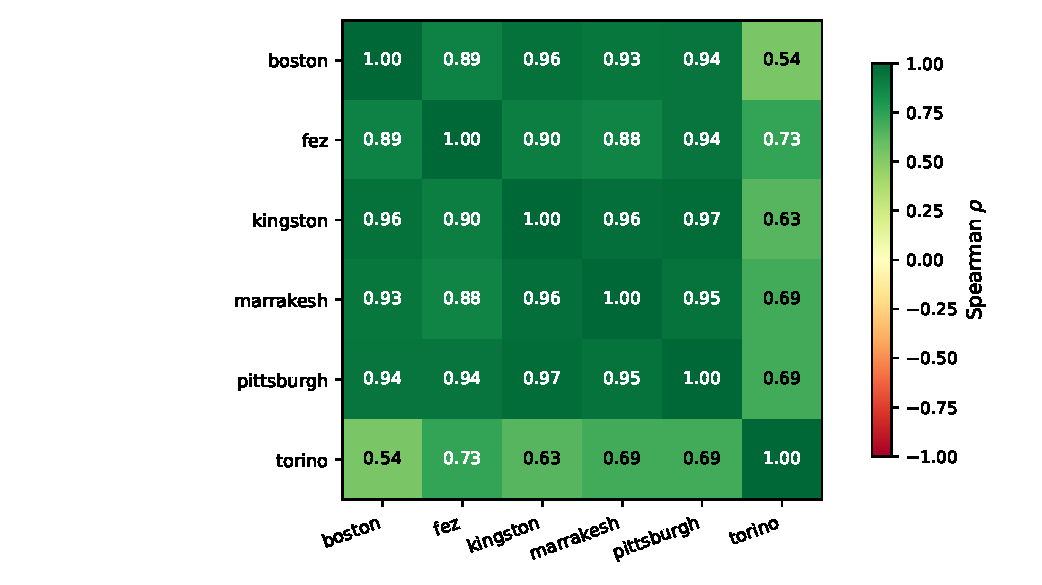
\includegraphics[width=0.72\textwidth]{fig5_cross_backend_corr.pdf}
\caption{Pairwise Spearman rank correlation of workload difficulty across backends. Most backend pairs show $\rho > 0.8$, except \texttt{ibm\_torino}, whose anomalous readout error decorrelates it from the others.}
\label{fig:crosscorr}
\end{figure*}

\begin{center}
\begin{minipage}{\columnwidth}
\refstepcounter{table}\label{tab:qft}
\small
\textbf{TABLE~\thetable.} QFT output entropy and collision probability by backend (v1.1~S1, 2\,048 shots; bootstrap SE on entropy $\leq 0.03$~bits). Ideal QFT-4 entropy: 4.0 bits; ideal QFT-5 entropy: 5.0 bits.

\begin{tabular}{lcccc}
\toprule
 & \multicolumn{2}{c}{QFT-4} & \multicolumn{2}{c}{QFT-5} \\
\cmidrule(r){2-3}\cmidrule(l){4-5}
Backend & $H$ (bits) & Coll. & $H$ (bits) & Coll. \\
\midrule
ibm\_boston     & 3.988 & 0.064 & 4.907 & 0.035 \\
ibm\_fez       & 3.973 & 0.065 & 4.883 & 0.037 \\
ibm\_kingston  & 3.989 & 0.063 & 4.963 & 0.033 \\
ibm\_marrakesh & 3.983 & 0.064 & 4.986 & 0.032 \\
ibm\_pittsburgh& 3.984 & 0.064 & 4.972 & 0.032 \\
ibm\_torino    & 3.966 & 0.065 & 4.954 & 0.033 \\
\bottomrule
\end{tabular}
\end{minipage}
\end{center}

For QFT circuits (Table~\ref{tab:qft}), output entropies approach the ideal uniform values across all backends, indicating that the measured distributions are close to the expected flat output. For fixed-seed random circuits, Shannon entropy and collision probability (mean over 4~seeds per width/depth bucket) are reported in the ancillary summary.

The VQE-H$_2$ sector fidelity (Table~\ref{tab:variational}) ranges from~0.82 (\texttt{ibm\_torino}) to~0.99 (\texttt{ibm\_boston}), with all six backends now reporting. The ranking is consistent with the CHSH and mirror workloads: the same devices that show lower readout fidelity also degrade VQE performance. The QAOA approximation ratios cluster at $r_{\text{approx}} \in [0.70,\, 0.74]$ (ideal~$0.75$), consistent with the fixed QASM-defined workload preserving the expected shallow-circuit behavior on real hardware; the narrow cross-backend spread ($\Delta r < 0.04$) reflects the shallow transpiled depth ($d{=}7$~two-qubit layers). These structured fixed-parameter probes are directionally consistent with the IBM-only ranking signal, but they should not be read as standalone variational experiments.

\begin{center}
\begin{minipage}{\columnwidth}
\refstepcounter{table}\label{tab:variational}
\small
\textbf{TABLE~\thetable.} Fixed-parameter structured-circuit results by backend (v1.1~S1, 2\,048~shots). VQE-H$_2$ reports sector fidelity $P(|01\rangle){+}P(|10\rangle)$ for the fixed-parameter 2-qubit UCCSD workload. QAOA-MaxCut4 reports approximation ratio $\langle C\rangle / C_{\max}$ for the fixed-parameter $p{=}1$ QAOA workload on $C_4$ ($C_{\max}{=}4$). Ideal values are from noiseless statevector simulation. Shot-noise SE $\leq 0.011$ for VQE and $\leq 0.012$ for QAOA.

\begin{tabular}{lcc}
\toprule
Backend & VQE $F_{\text{sec}}$ & QAOA $r_{\text{approx}}$ \\
\midrule
\textit{Ideal} & \textit{1.000} & \textit{0.750} \\
\midrule
ibm\_boston     & 0.985 & 0.734 \\
ibm\_fez       & 0.903 & 0.730 \\
ibm\_kingston  & 0.908 & n/a \\
ibm\_marrakesh & 0.938 & 0.724 \\
ibm\_pittsburgh& 0.905 & 0.742 \\
ibm\_torino    & 0.820 & 0.702 \\
\bottomrule
\end{tabular}
\end{minipage}
\end{center}

\subsection{Confirmatory stage (v1.1 Stage~S2)}
\label{sec:s2}

To address whether 2\,048~shots were sufficient, we executed a confirmatory subset at 8\,192~shots ($4\times$ S1) on 2~backends (\texttt{ibm\_marrakesh}, \texttt{ibm\_pittsburgh}). Coverage: 40/40 runs completed, all with binding verified. The confirmatory subset spans 10~circuit kinds (Mirror-1Q at 5~depths, GHZ-7, and 4~random-w6-d16 seeds) with 2~independent runs each. For all 10~circuit kinds, the S2 primary metric falls within the S1 shot-noise 95\% confidence interval ($\pm 1.96\sqrt{p(1{-}p)/N}$ with $N{=}2{,}048$); the full S1--S2 comparison table is in the ancillary data. This quantitative consistency supports the adequacy of the S1~evidence base.

%%% ---------------------------------------------------------------
\section{Noise-Model Comparison}
\label{sec:noisemodel}

To contextualize the raw CHSH results, we derive a depolarizing noise-model prediction and compare it to observations.

\textbf{Proposition~1} (Depolarizing CHSH bound). \emph{Let $\mathcal{E}_{\text{dep}}(\rho) = (1-\epsilon)\rho + \epsilon \, I/d$ act on the two-qubit gate with error rate~$\epsilon_{2q}$, and let each qubit undergo symmetric readout bit-flip with probability~$\epsilon_{\text{ro}}$. Neglecting single-qubit gate errors, the noisy CHSH parameter satisfies}
\begin{equation}
  S_{\text{noisy}} = 2\sqrt{2} \, (1 - \epsilon_{2q}) \, (1 - 2\epsilon_{\text{ro}})^2\,.
  \label{eq:noisemodel}
\end{equation}

\emph{Proof sketch.} The ideal Bell state $|\Phi^+\rangle$ yields parity correlation $E(\theta_a, \theta_b) = \cos(\theta_a - \theta_b)$ and $S = 2\sqrt{2}$. A depolarizing channel with parameter $\epsilon_{2q}$ maps the density matrix as $\rho \mapsto (1-\epsilon_{2q})\rho + \epsilon_{2q} I/4$. The maximally mixed component contributes zero to all correlations, so $E \to (1-\epsilon_{2q})\, E$. The Bell-state preparation circuit contains one CX/ECR gate, the sole two-qubit gate, and one H~gate (whose single-qubit error we neglect), yielding an attenuation factor of $(1-\epsilon_{2q})$. Symmetric readout error with probability $\epsilon_{\text{ro}}$ per qubit flips each measurement outcome independently, mapping parity expectation $E \to (1-2\epsilon_{\text{ro}})^2 E$ for the two-qubit system. Combining: $S_{\text{noisy}} = 2\sqrt{2}(1-\epsilon_{2q})(1-2\epsilon_{\text{ro}})^2$. \hfill$\square$

\noindent This result follows from standard depolarizing-channel algebra (see, e.g., Ref.~\cite{Gambetta2017}); we state it as a formal proposition to make the assumptions explicit, falsifiable, and directly comparable to the measured data below.

\textbf{Assumptions and scope.} Proposition~1 assumes (i)~the depolarizing channel dominates over coherent errors (e.g., over-rotation, residual ZZ coupling), (ii)~single-qubit gate error is negligible relative to two-qubit gate error, (iii)~readout errors are symmetric ($P(\text{flip}|0) \approx P(\text{flip}|1)$) and independent across qubits, and (iv)~the published gate error rate~$\epsilon_{2q}$ approximates the depolarizing parameter (the exact conversion $d^2/(d^2{-}1) = 16/15$ introduces a ${\lesssim}0.1\%$ correction absorbed into systematic uncertainty). Real IBM devices exhibit asymmetric readout errors ($P(1|0) \neq P(0|1)$); the symmetric approximation is a first-order model. For the five Eagle~r3 backends, the resulting bias in predicted~$S$ is estimated at $\lesssim 0.05$, subdominant to the larger model residuals discussed below, but may account for a non-negligible fraction of the \texttt{ibm\_torino} discrepancy. Deviations from these assumptions, particularly coherent errors and crosstalk, produce residuals not captured by Eq.~(\ref{eq:noisemodel})~\cite{Sarovar2020}.

\textbf{Comparison to data.} Using published median gate and readout error rates from IBM's backend calibration data~\cite{IBM2024} (snapshot: January 28, 2026; all runs were executed within a two-week window centered on this calibration date, using the specific qubit pairs from our CHSH circuits), the gate-plus-readout model matches observed mean~$S$ within 3\% for 3 of 6 backends (\texttt{ibm\_boston}, \texttt{ibm\_kingston}, and \texttt{ibm\_marrakesh}; Fig.~\ref{fig:noisemodel}). For the remaining three backends (\texttt{ibm\_pittsburgh}, \texttt{ibm\_fez}, and \texttt{ibm\_torino}), residuals are substantially larger ($-0.18$, $-0.26$, and $-0.36$ respectively), indicating that the simple depolarizing-plus-readout model is inadequate on these devices and that additional error sources, including coherent effects such as residual ZZ coupling, likely matter~\cite{Gambetta2017}. The model is therefore best read as a deliberately simple stress test: where it succeeds, published gate/readout figures explain CHSH at first order; where it fails, the residuals localize missing physics that a richer model must capture.

The model predicts \texttt{ibm\_torino}'s CHSH failure: with $\epsilon_{\text{ro}} \approx 0.045$, $S_{\text{noisy}} \approx 2.33$, above the classical bound but below the observed $S \approx 1.97$. This $-0.36$ residual decomposes approximately as $-0.15$ attributable to the elevated readout error (already captured) and $-0.21$ to unmodeled noise channels, consistent with the Heron~r2 processor's known susceptibility to ZZ crosstalk at higher qubit densities~\cite{Sarovar2020}. The model should therefore be read as a partial baseline rather than as a general predictive account of backend behavior.

\begin{figure}[tb]
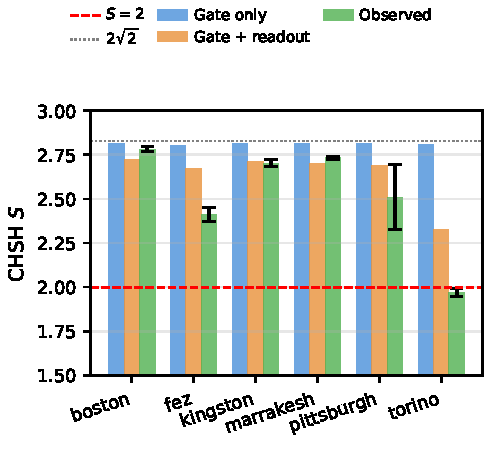
\includegraphics[width=\columnwidth]{fig4_noise_model.pdf}
\caption{Observed vs.\ predicted CHSH $S$ across 6 backends. Blue bars show the gate-only model, orange bars the gate-plus-readout depolarizing model, and green bars the observed mean with $\sigma$ error bars. The red dashed line marks the classical bound and the gray dotted line marks the Tsirelson bound. The gate-plus-readout model matches observations to within 3\% on 3~backends; \texttt{ibm\_torino}'s large readout error ($\epsilon_{\text{ro}} \approx 0.045$) dominates its below-threshold $S$.}
\label{fig:noisemodel}
\end{figure}

%%% ---------------------------------------------------------------
\section{Error Mitigation Case Study: \texttt{ibm\_torino}}
\label{sec:mitigation}

The noise-model comparison identifies readout error as the primary cause of \texttt{ibm\_torino}'s CHSH failure. To test this hypothesis, we apply matrix-free measurement mitigation (M3-style~\cite{Nation2021}) to the raw per-setting distributions. Each qubit's $2{\times}2$ confusion matrix is constructed from the symmetric readout error rate ($\epsilon_{\text{ro}} = 0.045$), tensored for the 2-qubit system, inverted, and applied to the observed probability vectors.

Post-mitigation, all three Bell-state runs on \texttt{ibm\_torino} recover CHSH violation: $S_{\text{mit}} \in [2.35,\, 2.40]$ with $\mathrm{CI}_{95,\text{low}} > 2.3$ in all cases. The negative-control (product-state) run correctly remains below $S = 2$ after mitigation ($S_{\text{mit}} \approx 1.18$). This demonstrates that (i)~the framework's declared claim gate correctly identified a readout-dominated failure rather than a genuine absence of entanglement, and (ii)~simple M3-style mitigation suffices to recover the expected physics.

We emphasize that all claim-gate verdicts in this paper are based on \emph{unmitigated} data, consistent with the declared analysis plan. The mitigation analysis is presented as a \emph{diagnostic} that explains the negative result, not as a post-hoc rescue.

%%% ---------------------------------------------------------------
\section{Bootstrap Validation of IID Confidence Intervals}
\label{sec:bootstrap}

The IID analytic confidence intervals (Sec.~\ref{sec:reproducibility}) assume independent shots. To validate this assumption, we perform non-parametric bootstrap resampling~\cite{Efron1979} ($B = 10{,}000$ replicates) of the per-setting shot data for all 33~CHSH runs. For each replicate, we resample $N$ outcomes with replacement from each measurement setting and recompute~$S$.

The mean ratio of bootstrap CI~width to IID CI~width is $0.997$ (range: $0.983$--$1.014$), confirming that the IID approximation is adequate for these workloads at these shot counts. No run shows a bootstrap/IID ratio exceeding~$1.05$, providing quantitative evidence that temporal correlations (T1/T2 drift, TLS fluctuators) do not significantly inflate uncertainty at $N \leq 16{,}384$ shots. We note that this validation applies to the specific backends and calibration windows tested; future work should apply Allan variance analysis~\cite{Sarovar2020} to characterize longer-timescale drift.

%%% ---------------------------------------------------------------
\section{Scaling Analysis: GHZ Parity vs.\ Qubit Count}
\label{sec:scaling}

To extract a physics result from the workload expansion data, we model the GHZ parity success $P_{\text{parity}} = P(0^n) + P(1^n)$ using the exponential decay ansatz:
\begin{equation}
  P_{\text{parity}}(n) = A \cdot (1 - 2p)^n
  \label{eq:ghzscaling}
\end{equation}
where $p$ is the effective per-qubit depolarizing error rate and $A$ is a prefactor accounting for state-preparation and readout fidelity.

\textbf{Mirror-to-GHZ-7 exponential diagnostic.} The bundled verifier fits each backend using Mirror-1Q ($n{=}1$, measuring readout fidelity $P(0)$) and GHZ-7 (measuring multi-qubit parity). The GHZ-3 and GHZ-5 remediation measurements are reported in Table~\ref{tab:ghz_grover}; the current reproducibility script treats the $n{=}1$ and $n{=}7$ points as a descriptive two-point diagnostic rather than as a goodness-of-fit test. We fit via least-squares minimization of $\log P_{\text{parity}}(n)$ versus $n$.

From this diagnostic fit, the extracted error rates range from $p = 0.006$ (\texttt{ibm\_marrakesh}) to $p = 0.054$ (\texttt{ibm\_fez}), spanning nearly an order of magnitude (Fig.~\ref{fig:ghzscaling}). The \texttt{ibm\_torino} effective error ($p = 0.021$) is dominated by its readout contribution, consistent with the Mirror-1Q baseline ($P(0) \approx 0.91$). For the three backends where the depolarizing model matches CHSH data within 3\% (Sec.~\ref{sec:noisemodel}), the extracted $p$ values are consistent with independently measured randomized-benchmarking error rates in the literature~\cite{Proctor2021,Magesan2011}, lending physical credibility to the exponential ansatz while remaining a descriptive estimate rather than a formal model-selection result.

\begin{figure*}[tb]
\centering
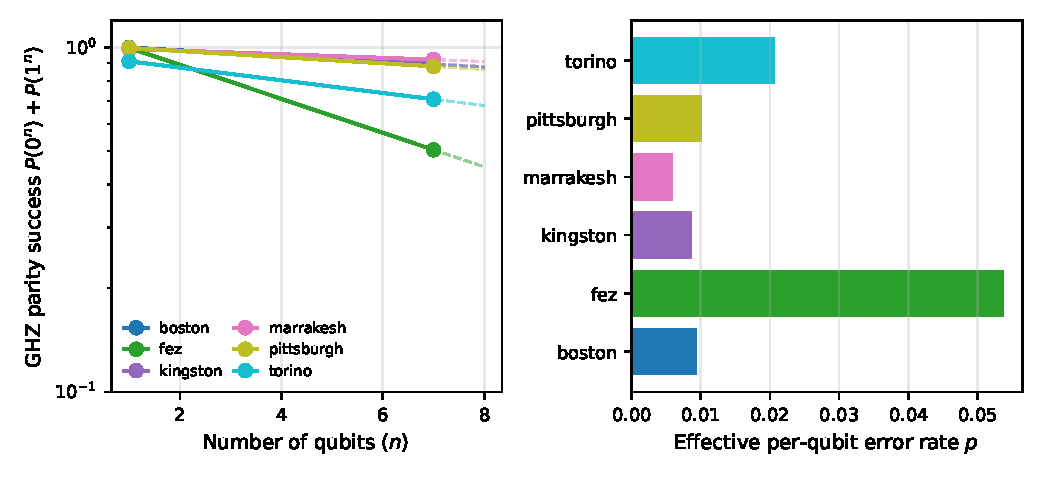
\includegraphics[width=0.9\textwidth]{fig6_ghz_scaling.pdf}
\caption{Left: GHZ parity success diagnostic with exponential fit $P(n) = A(1{-}2p)^n$ using the bundled Mirror-1Q and GHZ-7 points. Right: extracted descriptive per-qubit error rate by backend.}
\label{fig:ghzscaling}
\end{figure*}

%%% ---------------------------------------------------------------
\section{Discussion}
\label{sec:discussion}

\subsection{Physical interpretation of results}

The extracted per-qubit error rates ($p = 0.006$--$0.054$) span the range reported by independent randomized benchmarking studies on IBM Eagle~r3 processors~\cite{Proctor2021,Magesan2011}. That the same order of magnitude emerges from the bundled Mirror-to-GHZ-7 exponential diagnostic (Sec.~\ref{sec:scaling}) as from RB suggests that the ansatz $P(n) \propto (1-2p)^n$ captures a dominant component of the observed degradation.

The central finding of this paper is a stable workload-ordering signal within the IBM corpus ($\bar{\rho} = 0.84$ overall, $\bar{\rho} = 0.93$ excluding \texttt{ibm\_torino}) across the 28 complete six-backend workload kinds that span four qualitatively distinct circuit families: entanglement witnesses (GHZ-7), identity-equivalent diagnostics (mirror), algebraic transforms (QFT, Grover), and variational ansätze (VQE-H$_2$, QAOA-MaxCut). That the correlation persists across families, not merely within parametric sweeps of a single circuit, is consistent with a substantial workload-structure signal for circuits with depth $\lesssim 20$ on the IBM devices tested here. It is also consistent with a weaker explanation, namely that closely related IBM devices with shared software and calibration practice preserve similar rankings. The present paper does not discriminate cleanly between those explanations. The weaker correlation of \texttt{ibm\_torino} (Heron~r2, mean $\rho \approx 0.65$ with Eagle backends) points to a qualitatively different noise profile, consistent with a larger contribution from readout error ($\epsilon_{\text{ro}} \approx 0.045$) and other unmodeled effects, that decorrelates its performance rank from the Eagle fleet.

The new internal hardening checks narrow one obvious reviewer concern without overstating what they prove. Leave-one-family-out recomputation keeps mean $\bar{\rho}$ between $0.77$ and $0.89$, leave-one-workload-out shifts it by at most $0.021$, and residualized rank correlations remain strongly positive after adjusting for workload width, QASM-derived logical depth proxy, and family. At the same time, the family-clustered bootstrap interval for mean $\bar{\rho}$ remains wide ($[0.44,\,0.96]$) because only seven workload families are available and their sizes are imbalanced. These checks strengthen the IBM-only regularity claim, but they do not remove the need for genuinely heterogeneous vendor data.

\textbf{Null hypothesis: architectural homogeneity.} The strongest alternative explanation for the high cross-backend correlation ($\bar{\rho} = 0.93$ among Eagle~r3) is that closely related processors naturally produce similar performance rankings, an artifact of \emph{architectural homogeneity} rather than intrinsic circuit complexity. The present single-vendor data do not reject that null. The partial decorrelation of \texttt{ibm\_torino} is suggestive but not decisive, because Eagle and Heron remain related IBM superconducting families with shared tooling and operating procedures. The added family/workload sensitivity checks are internal robustness tests, not direct tests of this architectural null. Accordingly, the cross-backend correlations reported here should be interpreted as an IBM-family empirical regularity, not as proof that circuit complexity is hardware-independent. A decisive test requires the same workload set on architecturally distinct vendor families under the stronger execution-identity contract described below.

\textbf{Comparison to existing benchmarks.} Our framework captures information orthogonal to Quantum Volume~\cite{Cross2019}: QV reports a single pass/fail threshold, whereas our corpus separates gate error from readout error, tracks per-workload difficulty, and provides workload-level provenance. For the same backends, IBM reports QV~$\geq 128$ for all six~\cite{IBM2024}, yet our data reveal an order-of-magnitude spread in effective error rates, information invisible to QV. Similarly, CLOPS measures throughput, not fidelity, and SupermarQ~\cite{Tomesh2022} does not require a public declared-plan surface at release time. Our framework's contribution is thus \emph{complementary}: it adds provenance, declared decision gates, and noise decomposition to existing benchmark suites.

\subsection{Framework value}

Without declared decision rules and confidence intervals, \texttt{ibm\_torino}'s $S \approx 1.98$ might be reported as a ``marginal pass'' or excluded. The framework's gate ($S > 2.0$ \emph{and} $\mathrm{CI}_{95,\text{low}} > 2.0$) classifies this unambiguously as a \emph{failure}, the noise model (Proposition~1) identifies readout error as the mechanism, and the mitigation analysis (Sec.~\ref{sec:mitigation}) confirms the diagnosis. This detect--explain--confirm sequence requires the provenance and analysis infrastructure described here.

\subsection{Limitations and future work}

This work has seven principal limitations. First, the statistical hardware corpus comes from IBM superconducting devices. Second, the evaluation plan is author-preserved rather than independently preregistered with a third-party timestamp. Third, provider job IDs provide job-id provenance but not provider-signed attestation. Fourth, the declared target scope differs from the completed public evidence scope (Table~\ref{tab:scope_reconciliation}); we preserve that distinction rather than rewriting historical declarations. Fifth, the current workload hashes bind logical OpenQASM bytes, not post-transpilation circuit identity, transpiler versions, physical layouts, or pulse schedules. Sixth, the bundled non-IBM evidence is a second-provider AWS Braket confirmation set rather than a matched multi-vendor statistical corpus; Azure-side simulator submissions are excluded from the real-hardware claim. Seventh, family-level uncertainty is still only coarsely resolved: the family-clustered bootstrap interval for mean $\bar{\rho}$ is wide because the current corpus contains only seven workload families with uneven family sizes. The GHZ scaling script is likewise a descriptive diagnostic rather than a formal model-selection test.

The author-declared evaluation plan is preserved in the public ancillary/release surface. The reconciled evidence capsule is released under Zenodo version DOI \href{https://doi.org/10.5281/zenodo.19985231}{10.5281/zenodo.19985231} within the release series identified by concept DOI \href{https://doi.org/10.5281/zenodo.19954163}{10.5281/zenodo.19954163}; the version DOI provides the stable package identifier, but it is a release timestamp rather than an independent pre-execution registry timestamp. For the next campaign, the evaluation-plan hash will be committed on day zero to a public repository surface and to an external transparency log such as Rekor or OpenTimestamps.

The GHZ scaling curve (Sec.~\ref{sec:scaling}) now includes $n{=}3,5,7$ (one residual degree of freedom); additional sizes ($n{=}9,11$) would further constrain the exponential fit. The $-0.36$ ibm\_torino residual (Sec.~\ref{sec:noisemodel}) warrants dedicated Heron~r2 characterization, potentially including process tomography and Allan variance analysis for temporal drift. The noise model (Proposition~1) treats gate errors as purely depolarizing; dedicated characterization of coherent error channels, via gate-set tomography~\cite{Merkel2013} or randomized benchmarking interleaved with crosstalk-sensitive gates, would enable a more refined predictive model. More broadly, the next decisive empirical upgrade is a matched multi-vendor corpus: the current AWS Braket confirmation set shows that the evidence contract survives on a second real-hardware provider surface, but it does not validate the full statistical corpus across architecturally distinct platforms. Any stronger follow-up should therefore prioritize vendor-diverse hardware coverage plus post-transpilation circuit hashes, transpiler versions, optimization levels, physical layouts, calibration snapshots, compiled/native programs, and provider-specific job metadata.

%%% ---------------------------------------------------------------
\section{Conclusion}
\label{sec:conclusion}

We find evidence that workload difficulty rankings are preserved within the IBM superconducting family studied here: pairwise Spearman correlations across 6~backends and 28~complete six-backend workload kinds, spanning mirror circuits, GHZ-7, Grover search, QFT, random circuits, fixed-parameter VQE, and fixed-parameter QAOA, yield $\bar{\rho} = 0.84$. Deterministic permutation sensitivity retains 14/15~Bonferroni-significant pairs, with \texttt{ibm\_boston}--\texttt{ibm\_torino} borderline; the analytic Spearman test gives 15/15~significant pairs. Leave-one-family-out and leave-one-workload-out perturbations preserve the signal, and residualized rank correlations remain strongly positive after adjusting for width, logical depth proxy, and family, although the family-clustered interval remains wide because only seven workload families are available. This finding, enabled by an evidence-first framework with content-addressed logical workloads and an author-preserved evaluation plan, is an IBM-only empirical regularity rather than evidence that circuit complexity is already known to be hardware-independent.

The paper's contribution is therefore twofold. First, it releases a reviewer-auditable evidence contract for NISQ benchmarking: public logical workloads, preserved decision rules, provider job-ID provenance, negative controls, and replayable analysis surfaces. Second, it demonstrates that contract on an IBM-only corpus whose cross-backend ranking structure survives several internal sensitivity checks while remaining explicitly bounded by single-vendor scope. The bundled AWS Braket confirmation set extends the evidence contract to a second real-hardware provider surface, but not to a matched multi-vendor statistical study. Broader claims about hardware-independent workload ordering require that stronger vendor-diverse follow-up.

%%% ---------------------------------------------------------------
\begin{acknowledgments}
This work was executed on IBM Quantum hardware via the IBM Quantum Network open plan. We acknowledge the open-source Qiskit community for the software stack and IBM Quantum for providing public access to superconducting processors. Backend availability and queue scheduling are provider-controlled; the backends used are recorded in the run tables.
\end{acknowledgments}

\section*{Data and Code Availability}

All workload definitions (full logical OpenQASM source + SHA256), execution manifests, and offline-recomputable distributions are included as public ancillary files and in the Zenodo release published under version DOI \href{https://doi.org/10.5281/zenodo.19985231}{10.5281/zenodo.19985231} within the release series identified by concept DOI \href{https://doi.org/10.5281/zenodo.19954163}{10.5281/zenodo.19954163}. A companion public commitment and receipt surface for this campaign is maintained in the public evidence-commitments repository (\href{https://github.com/invariant-systems-ai/evidence-commitments}{invariant-systems-ai/evidence-commitments}) at the \href{https://github.com/invariant-systems-ai/evidence-commitments/tree/main/commitments/nisq-readiness-2026-05-02}{NISQ campaign entry}; it mirrors the latest published paper-facing capsule and records the machine-readable commitment manifest plus the AIIR receipt bundles, Sigstore bundle sidecars, and Rekor-backed timestamps for the released packet. The concept DOI identifies the release series, while the current version DOI is a public release identifier rather than scientific evidence or an independent pre-execution registry timestamp. The key evidence tables are reproduced in this paper (Tables~\ref{tab:corpus_v10}--\ref{tab:variational}). No provider credentials or private repository access is required to verify the reported IBM statistical results. The release also includes \path{anc/22_AWS_BRAKET_REAL_HARDWARE_CONFIRMATION_20260501.md}, \path{anc/23_AWS_BRAKET_PROVIDER_FACTS_20260501.json}, and \path{anc/24_EXECUTION_ORDER_AND_TIMESTAMP_POSTURE_20260501.md}. Together, those companion surfaces record completed AWS Braket IQM Garnet confirmations, provider-side timestamps, logical hash fields, and the timestamp-boundary interpretation for the broader evidence contract. They support a narrow second-provider real-hardware portability claim for the evidence contract; they are not part of the IBM statistical dataset. Azure Quantum submissions from the same campaign were simulator-only under the attached workspace SKU and are excluded from the real-hardware claim. OpenQASM source for the VQE-H$_2$ and QAOA-MaxCut4 circuits is included in the ancillary bundle. The present release does not include post-transpilation circuit hashes, compiled/native programs for the IBM corpus, or physical-layout manifests; those are reserved for the planned multi-platform follow-up.

Ancillary scripts include: \texttt{verify\_chsh.py} (CHSH recomputation, stdlib only), \texttt{validate\_ancillaries.py} (schema validation), \texttt{noise\_model\_comparison.py} (depolarizing model predictions), \texttt{bootstrap\_ci.py} (bootstrap CI validation), \texttt{readout\_mitigation.py} (M3-style readout correction), \texttt{scaling\_analysis.py} (GHZ parity exponential diagnostic), \texttt{cross\_backend\_analysis.py} (Spearman correlation matrix), and \texttt{generate\_figures.py} (figure regeneration, requiring NumPy and Matplotlib). The release-local reproducibility guide lists the exact commands, inputs, outputs, and checksum instructions; those operational details should be treated as supplementary audit material rather than as part of the central scientific argument. The exported capsule and companion receipt surfaces were assembled with AIIR (\url{https://github.com/invariant-systems-ai/aiir}), but the scientific object of review is the released evidence package itself rather than the packaging toolchain.

\bibliography{references}

\end{document}
